\documentclass[11pt,a4paper]{article}

\usepackage{main}
\usepackage{exercices}

% --------------------------------------------------
% Informations du document
% --------------------------------------------------
\renewcommand{\typedocument}{Exercices}
\renewcommand{\classe}{5e}
\renewcommand{\titre}{Exercices - Série et dérivation}

\begin{document}

% ----- Exercice 1 -----

\exercice{Circuits en série et en dérivation}
Observer chaque schéma et indiquer s'il s'agit d'un circuit en série ou en dérivation.

\begin{minipage}{3cm}
    a.
    
    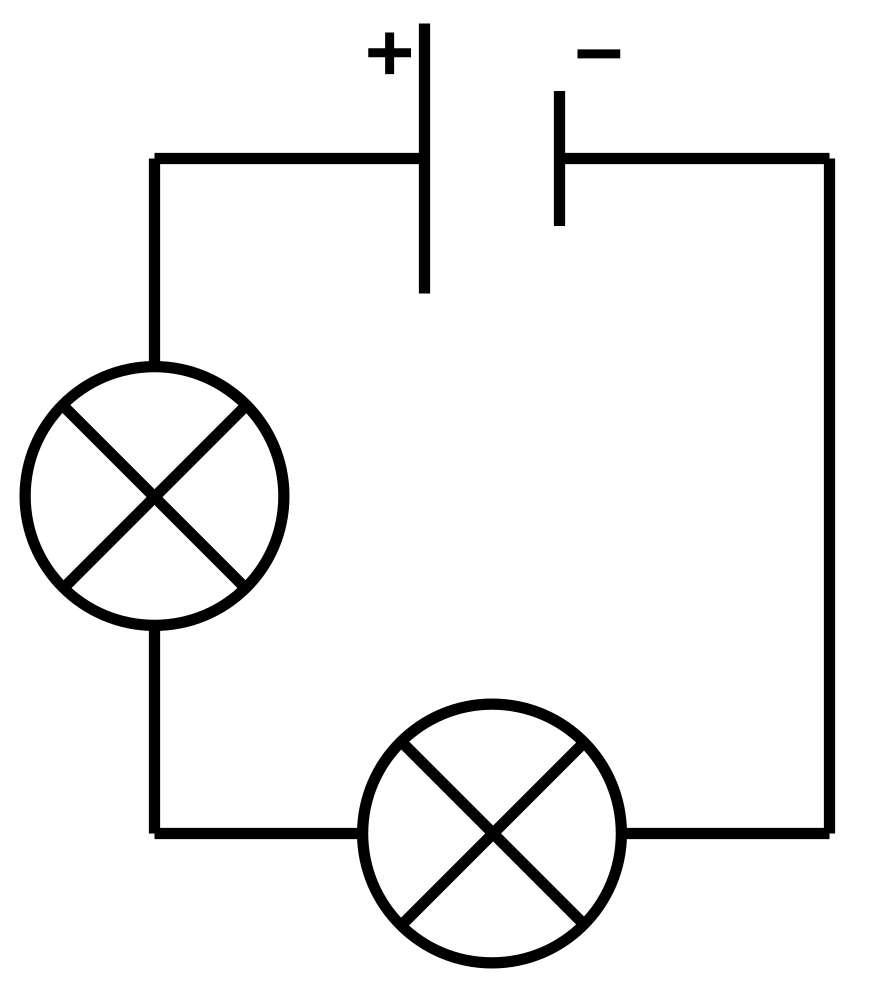
\includegraphics[width=3cm]{images/1a.png}
\end{minipage}
\hfill
\begin{minipage}{3.5cm}
    b. 
    
    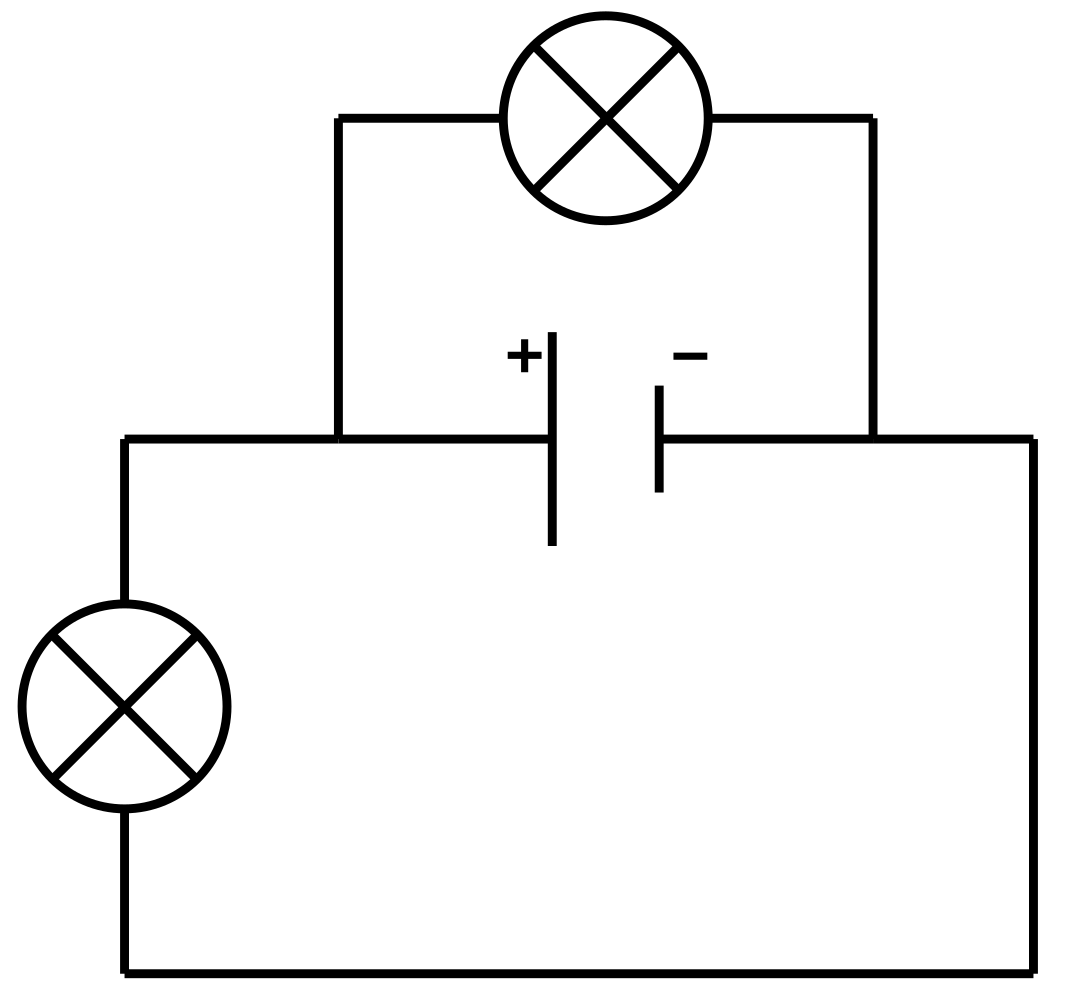
\includegraphics[width=3.5cm]{images/1b.png}
\end{minipage}
\hfill
\begin{minipage}{5cm}
    c.
    
    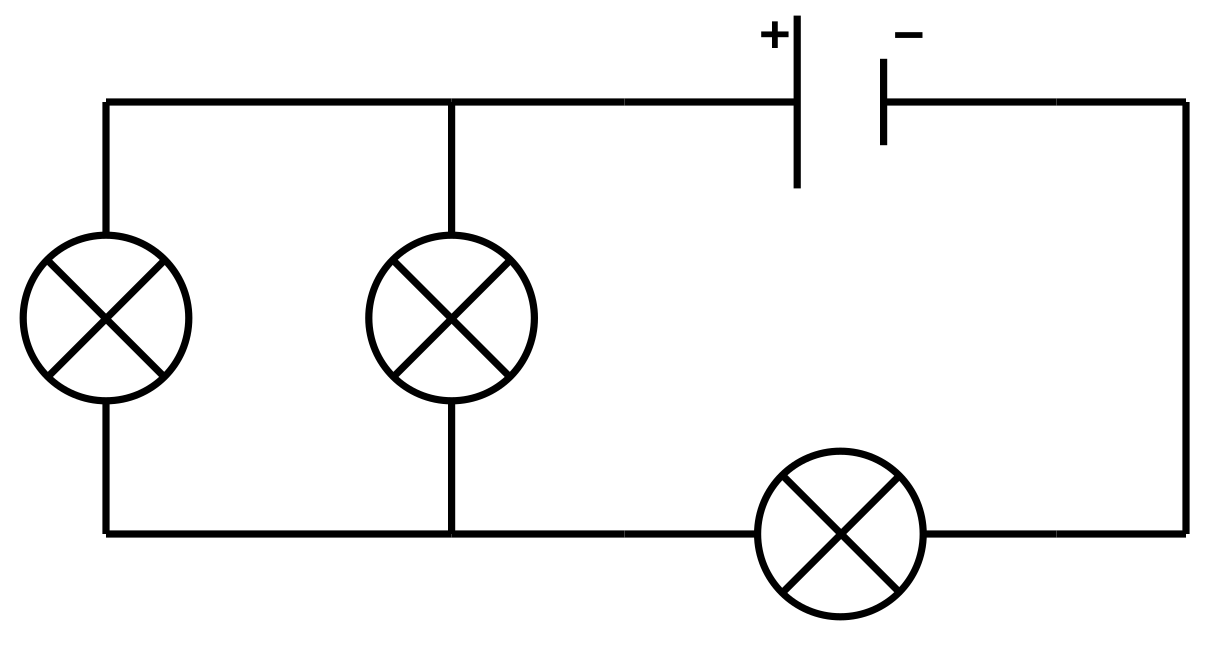
\includegraphics[width=5cm]{images/1c.png}
\end{minipage}
\hfill
\begin{minipage}{3cm}
    d.
    
    
\includegraphics[width=3cm]{images/1d.png}
\end{minipage}

% ----- Exercice 2 -----

\exercice{Courant et court-circuit}

Dans chacun des exemples suivants, surligner les fils par lesquels circule le courant et colorier les lampes allumées.

\begin{minipage}{3.5cm}
    a.
    
    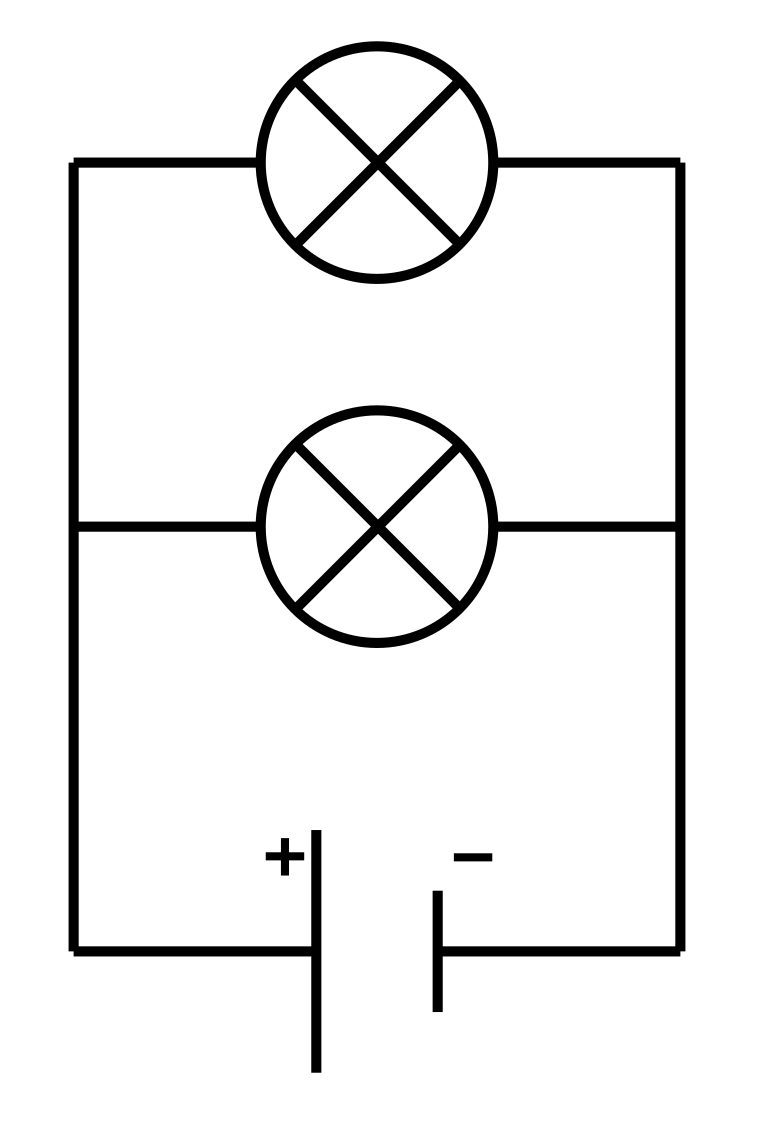
\includegraphics[width=3cm]{images/2a.png}
\end{minipage}
\hfill
\begin{minipage}{3.5cm}
    b. 
    
    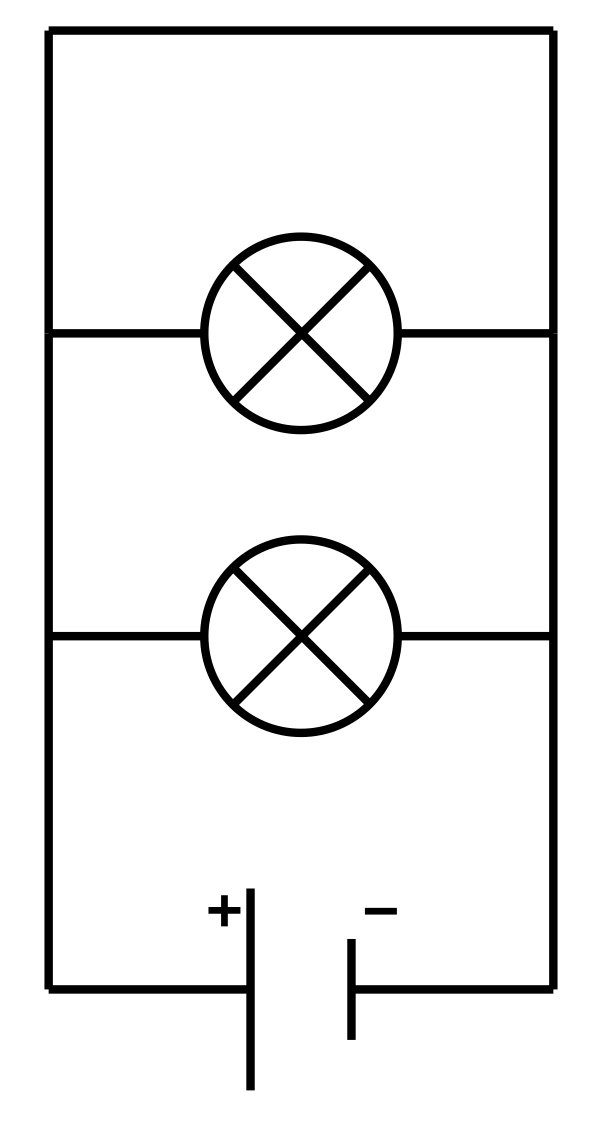
\includegraphics[width=3cm]{images/2b.png}
\end{minipage}
\hfill
\begin{minipage}{3.5cm}
    c.
    
    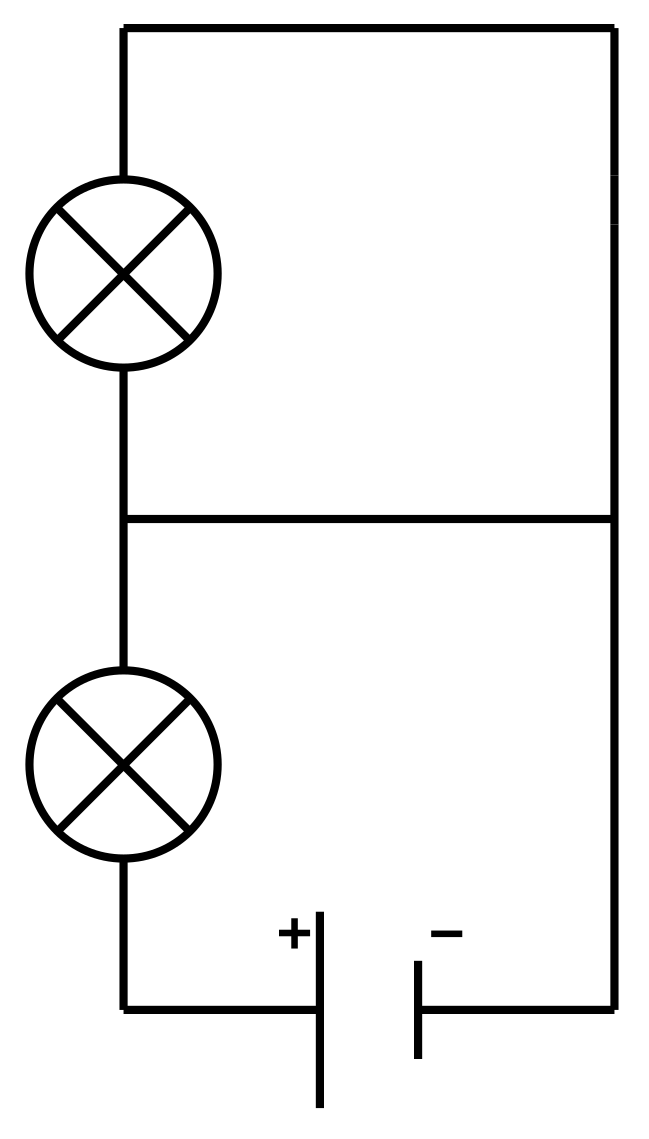
\includegraphics[width=3cm]{images/2c.png}
\end{minipage}
\hfill
\begin{minipage}{3.5cm}
    d.
    
    
\includegraphics[width=3cm]{images/2d.png}
\end{minipage}

% ----- Exercice 3 -----

\exercice{Interrupteur et court-circuit}

\begin{center}
    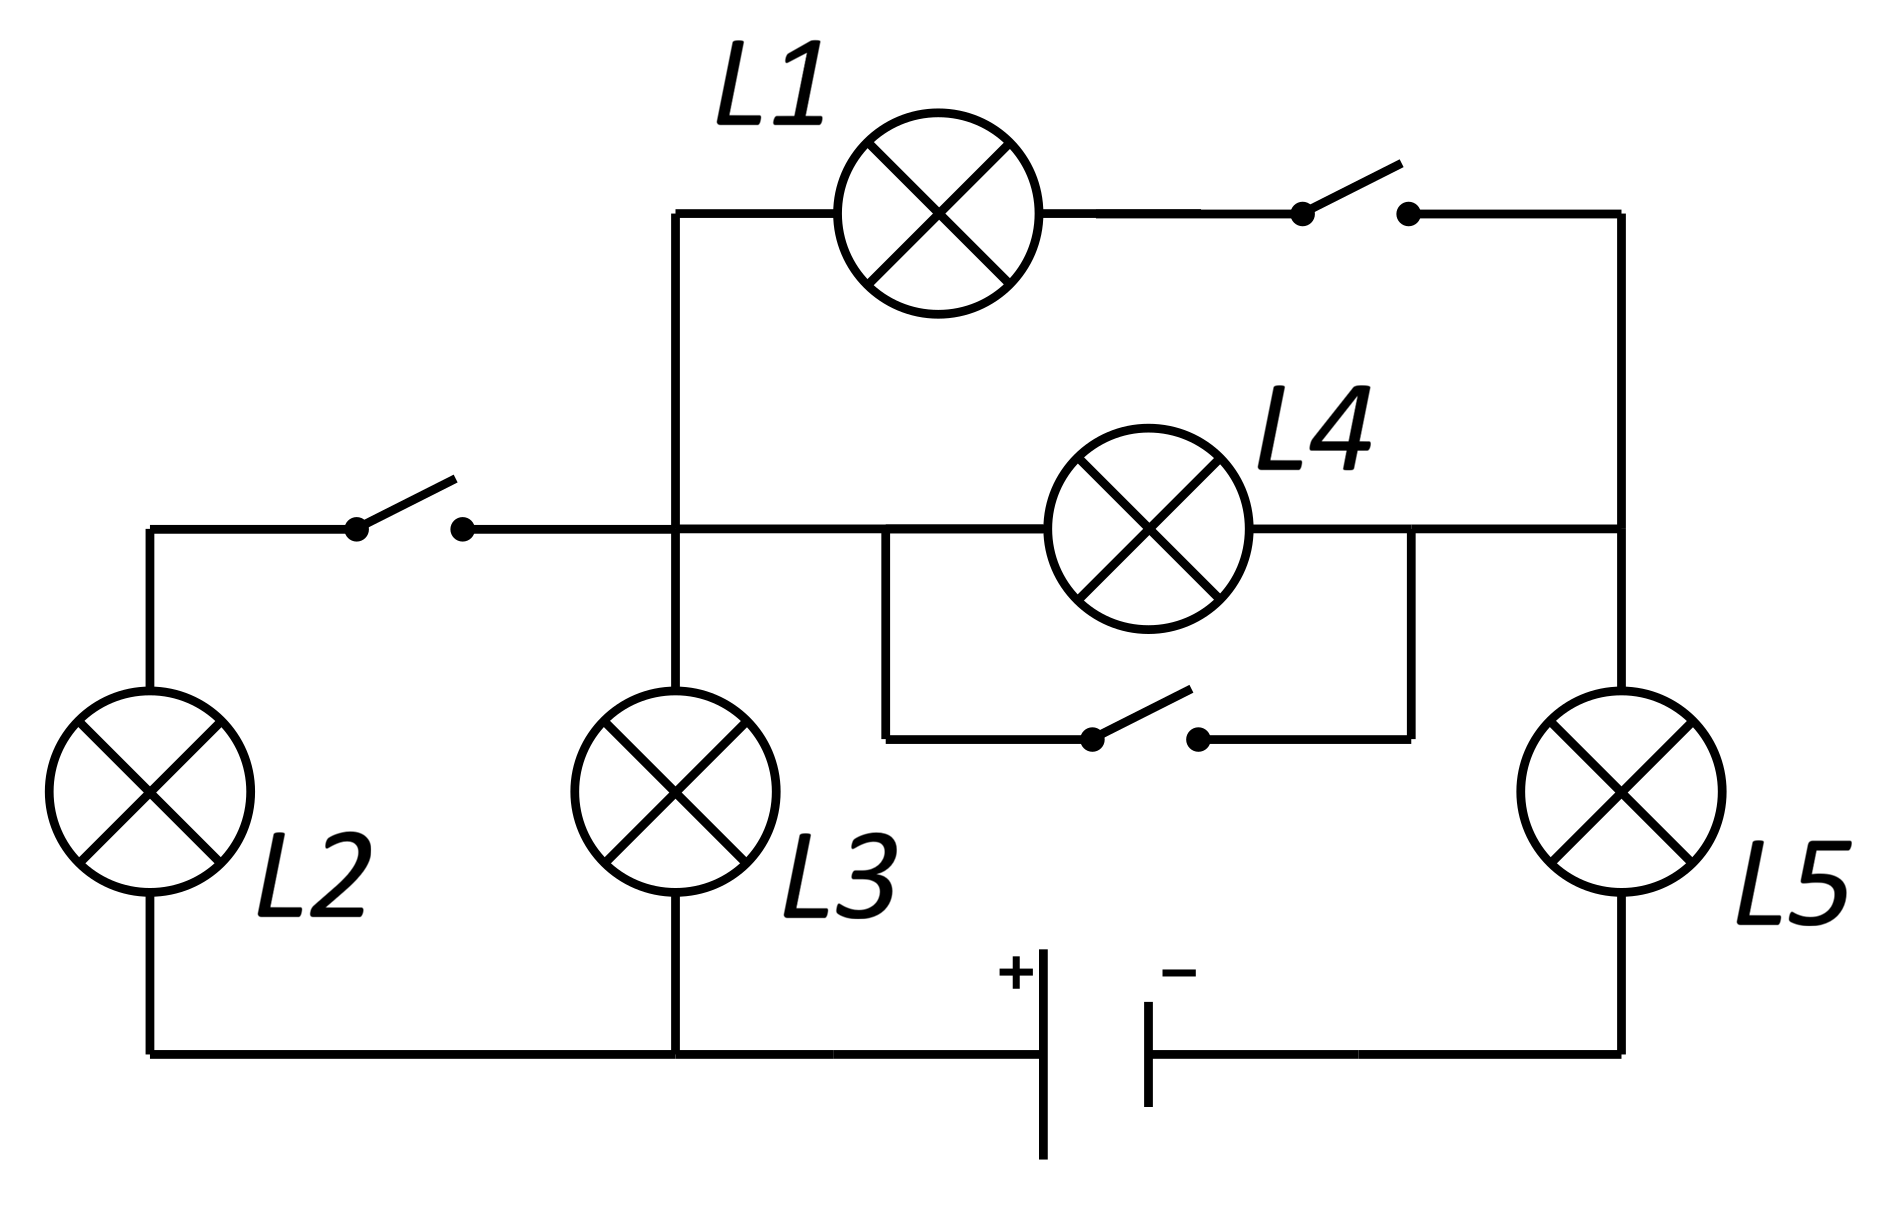
\includegraphics[width=9cm]{images/3.png}
\end{center}

\question{Quelles lampes sont allumées lorsque tous les interrupteurs sont ouverts ?}

\question{Quelles lampes sont allumées lorsque tous les interrupteurs sont fermés ?}

\newpage

% ----- Exercice 4 -----

\exercice{Intensité du courant}

\begin{minipage}{3.5cm}
    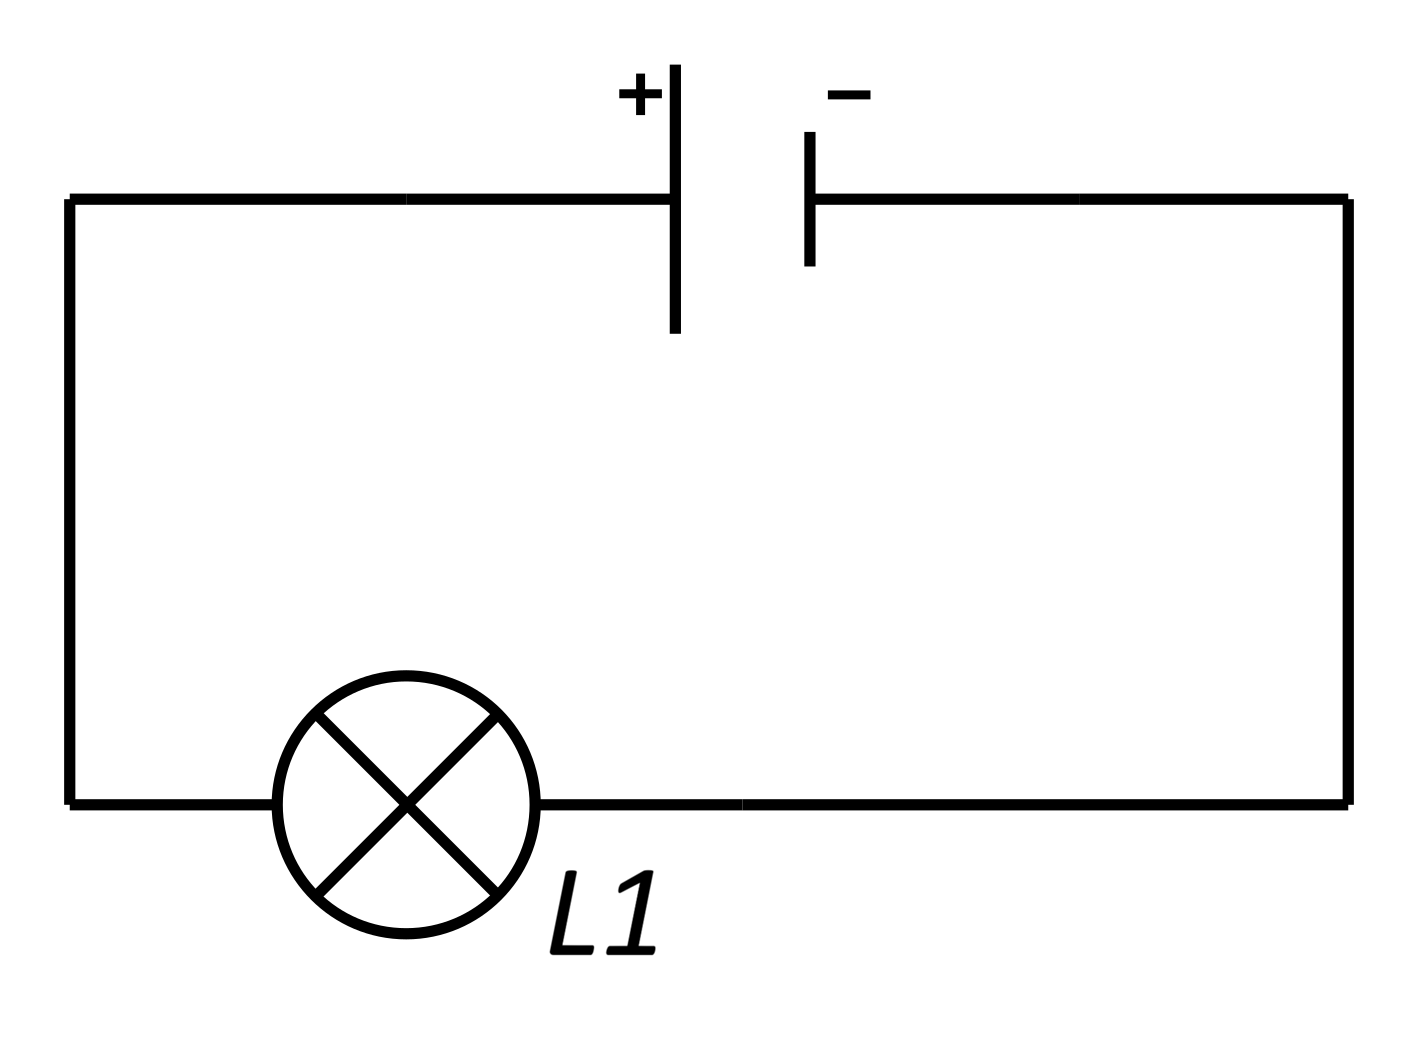
\includegraphics[width=3.5cm]{images/4a.png}
\end{minipage}
\hfill
\begin{minipage}{3.5cm}
    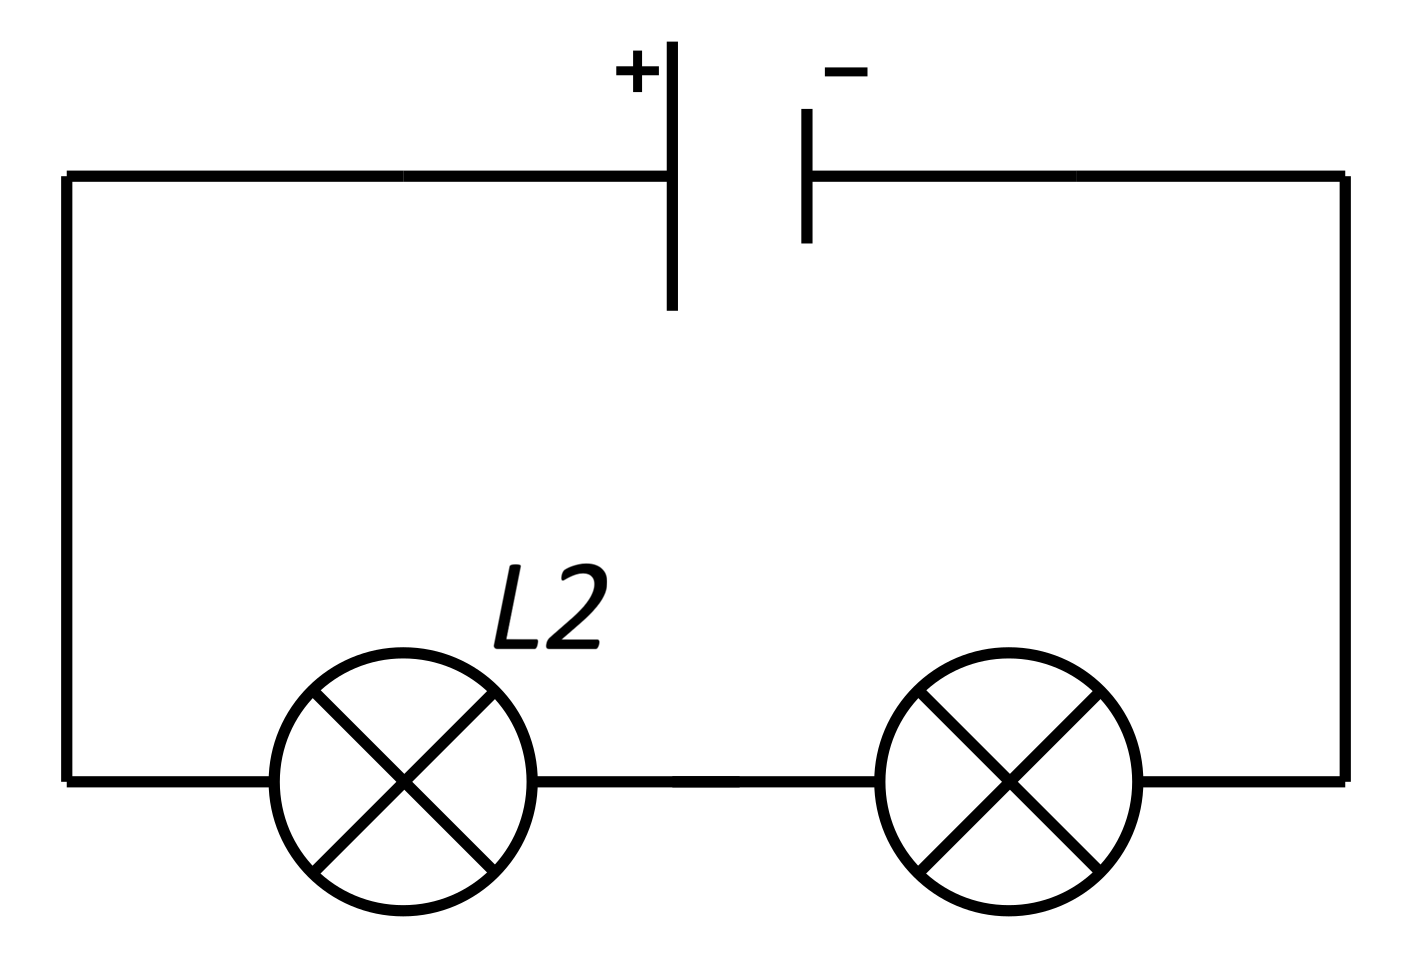
\includegraphics[width=3.5cm]{images/4b.png}
\end{minipage}
\hfill
\begin{minipage}{3.5cm}
    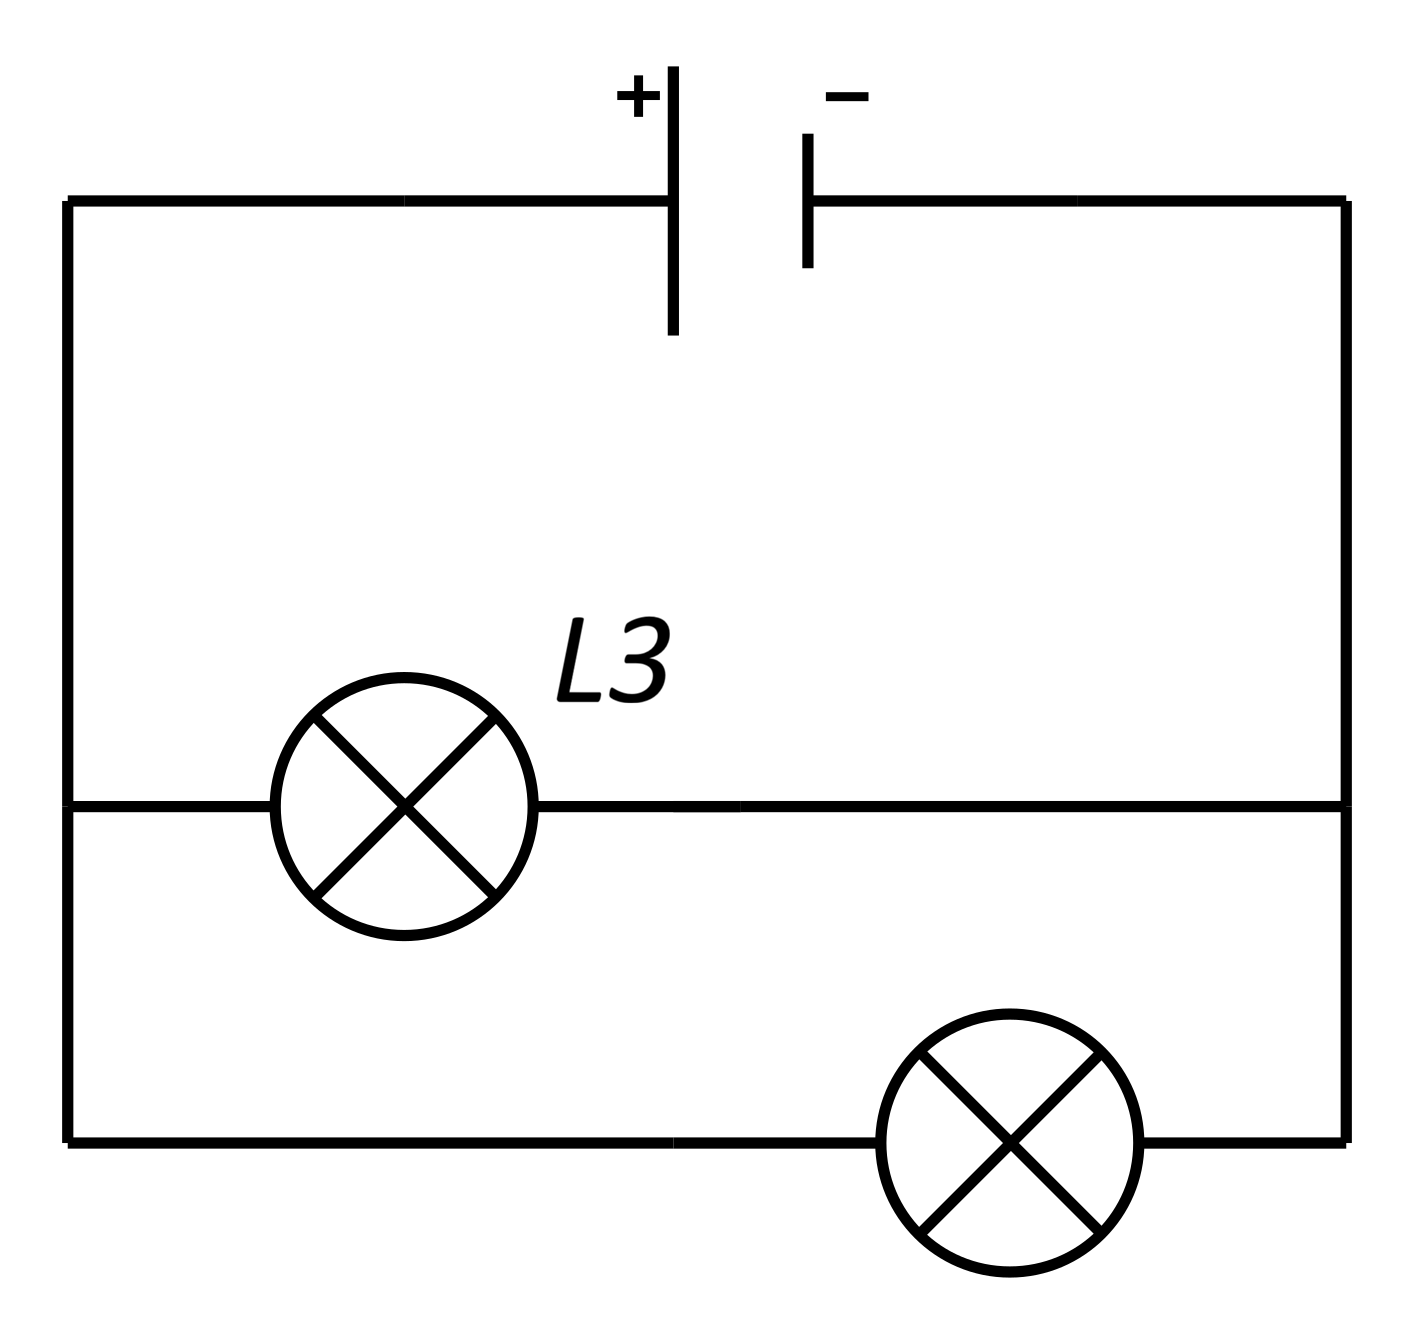
\includegraphics[width=3.5cm]{images/4c.png}
\end{minipage}
\hfill
\begin{minipage}{3.5cm}
    
\includegraphics[width=3.5cm]{images/4d.png}
\end{minipage}

Comparer les luminosités des lampes:
\begin{enumerate}
    \item L1 et L2,
    \item L1 et L3,
    \item L2 et L4.
\end{enumerate}

% ----- Exercice 5 -----

\exercice{Sécurité et court-circuit}

\question{Quels sont les risques d'un court-circuit ?}

\question{Pour chacun des circuits suivants, entourer les dipôles qui sont en court-circuit et surligner les fils qui relient leurs bornes.}

\begin{minipage}{8cm}
    a.
    
    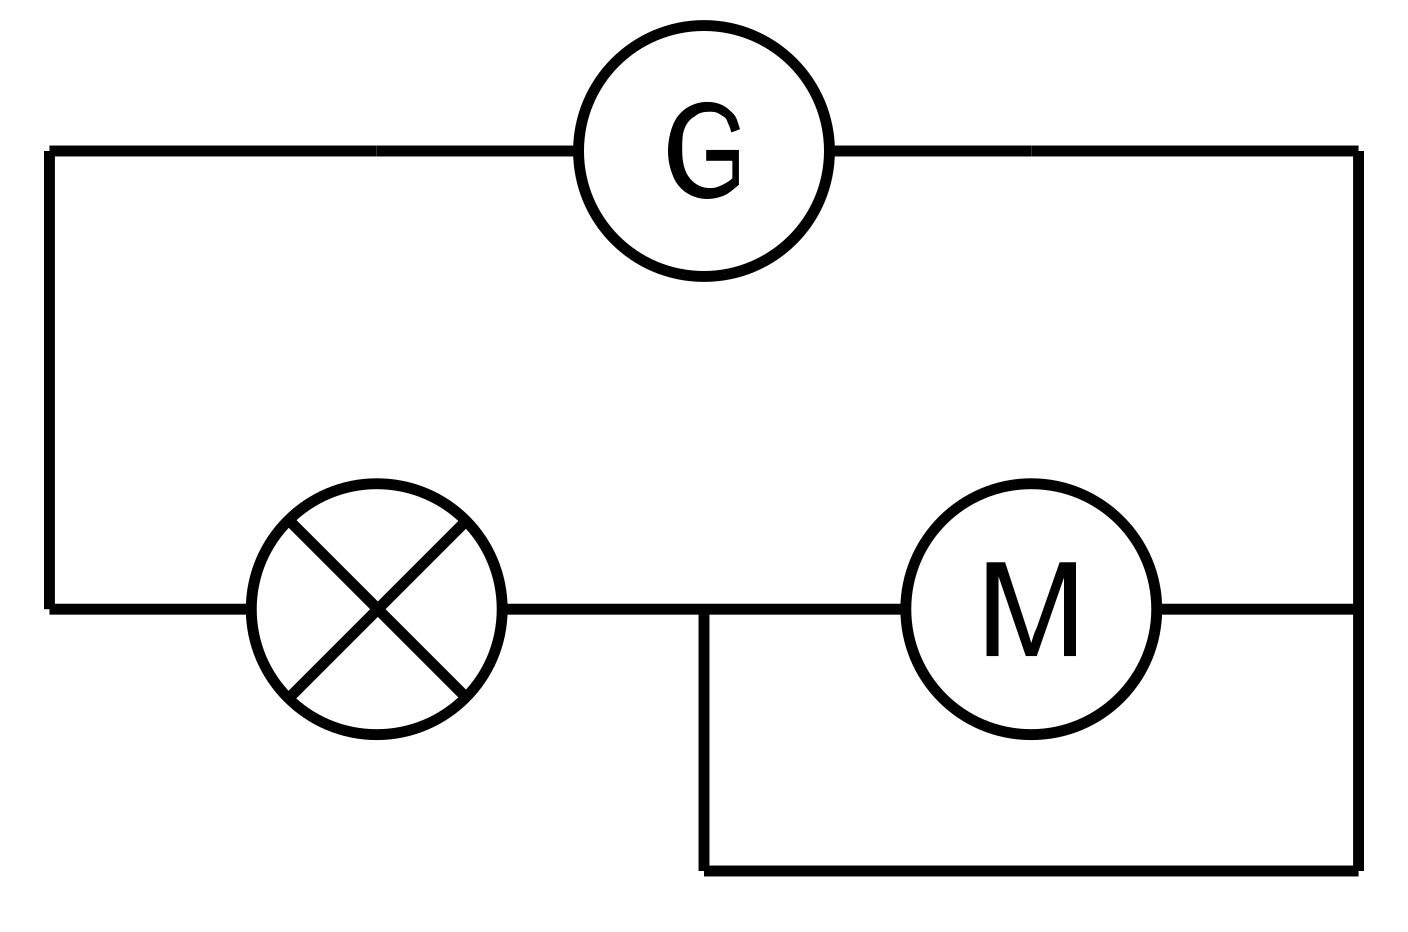
\includegraphics[width=8cm]{images/5a.png}
\end{minipage}
\hfill
\begin{minipage}{8cm}
    b. 
    
    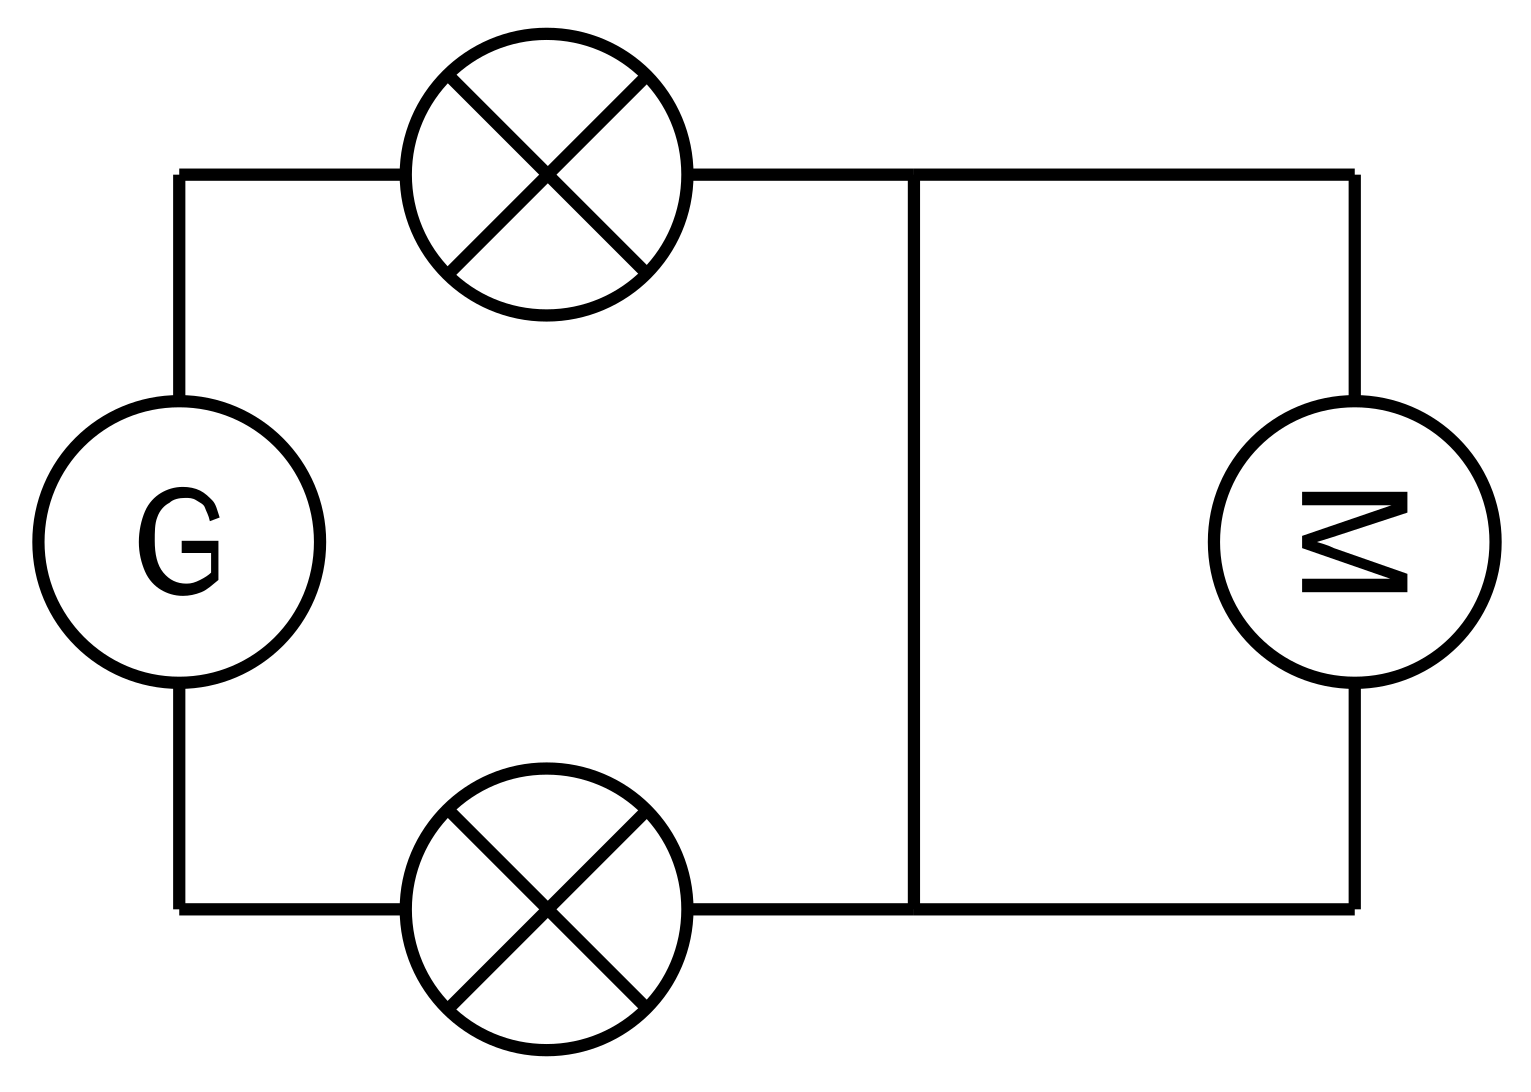
\includegraphics[width=8cm]{images/5b.png}
\end{minipage}

\begin{minipage}{8cm}
    c.
    
    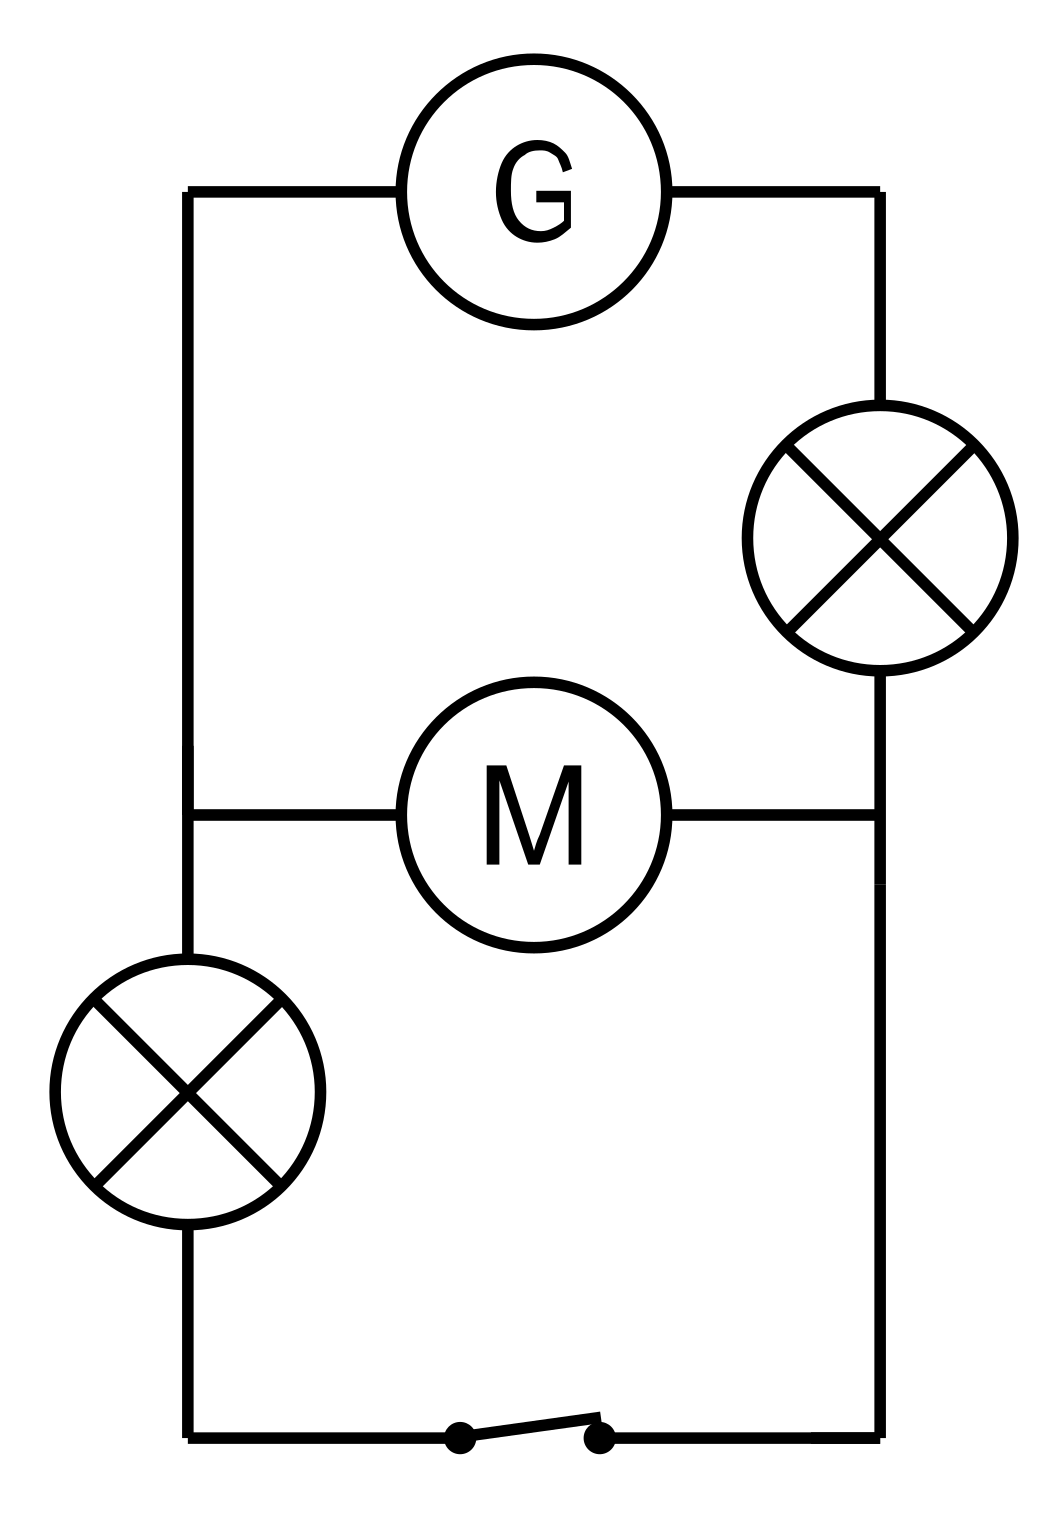
\includegraphics[width=6cm]{images/5c.png}
\end{minipage}
\hfill
\begin{minipage}{8cm}
    d.
    
    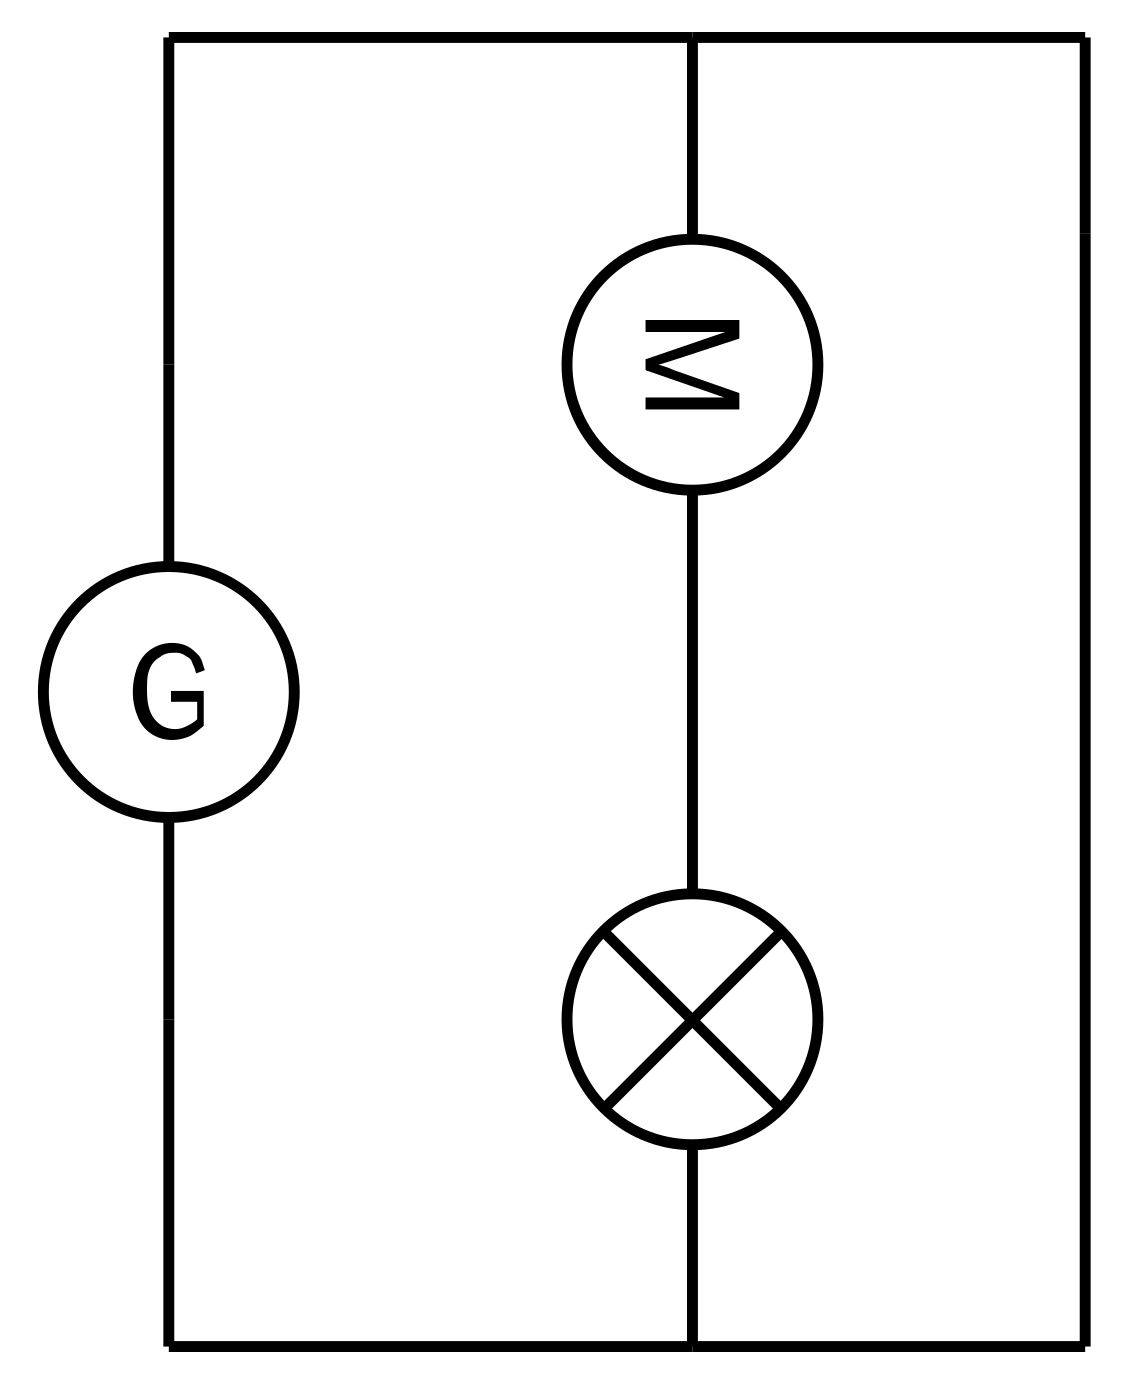
\includegraphics[width=6cm]{images/5d.png}
\end{minipage}

\question{Indiquer quel circuit est particulièrement dangereux et expliquer pourquoi.}

\end{document}